\documentclass[11pt,a4paper]{article}

\usepackage[T1]{fontenc}
\usepackage[utf8]{inputenc}
\usepackage[margin=0.9in]{geometry}
\usepackage{amsmath,amssymb}
\usepackage{tikz}
\usetikzlibrary{positioning,arrows.meta,calc,fit,backgrounds,shapes.misc}
\usepackage{xcolor}
\usepackage{booktabs}
\usepackage{microtype}
\usepackage{hyperref}
\hypersetup{colorlinks=true,linkcolor=blue,citecolor=blue,urlcolor=blue}

\definecolor{stable}{HTML}{1B7837}
\definecolor{unstable}{HTML}{C2272D}
\definecolor{neutralg}{HTML}{4D4D4D}
\definecolor{accent}{HTML}{2166AC}
\definecolor{accent2}{HTML}{B2182B}
\definecolor{fieldc}{HTML}{D9730D}
\definecolor{dropped}{HTML}{999999}

\tikzset{
  box/.style={rounded corners=2pt, draw=accent, fill=accent!7, align=center,
              inner sep=5pt, font=\small},
  goodbox/.style={rounded corners=2pt, draw=stable, fill=stable!9, align=center,
              inner sep=5pt, font=\small},
  badbox/.style={rounded corners=2pt, draw=unstable, fill=unstable!8, align=center,
              inner sep=5pt, font=\small},
  dropbox/.style={rounded corners=2pt, draw=dropped, fill=dropped!10, align=center,
              inner sep=5pt, font=\small, text=dropped},
  fieldbox/.style={rounded corners=2pt, draw=fieldc, fill=fieldc!12, align=center,
              inner sep=5pt, font=\small},
  >=Stealth,
}

\title{\vspace{-2em}Where we are\\[3pt]
\large A visual recap of the paradigm-dynamics rebuild\\
\normalsize (continuous substrate $\to$ categorical epistemic POMDP)}
\author{Internal recap --- IWAI 2026}
\date{2026-05-21}

\begin{document}
\maketitle
\vspace{-1.5em}

\noindent\textbf{One-sentence state:} we abandoned the continuous Gaussian model
(provably monostable), decided to rebuild as a categorical active-inference
POMDP, simplified it after a conversation with David (drop resource, fix the
hidden states, make ``theory'' a likelihood, make \emph{belief-utility} the
core), de-risked the bistability question, and built+tested the Phase-1
scaffold --- which surfaced one important wall (next page).

% =====================================================================
\section*{1.\quad The arc: what changed and why}
% =====================================================================
\begin{center}
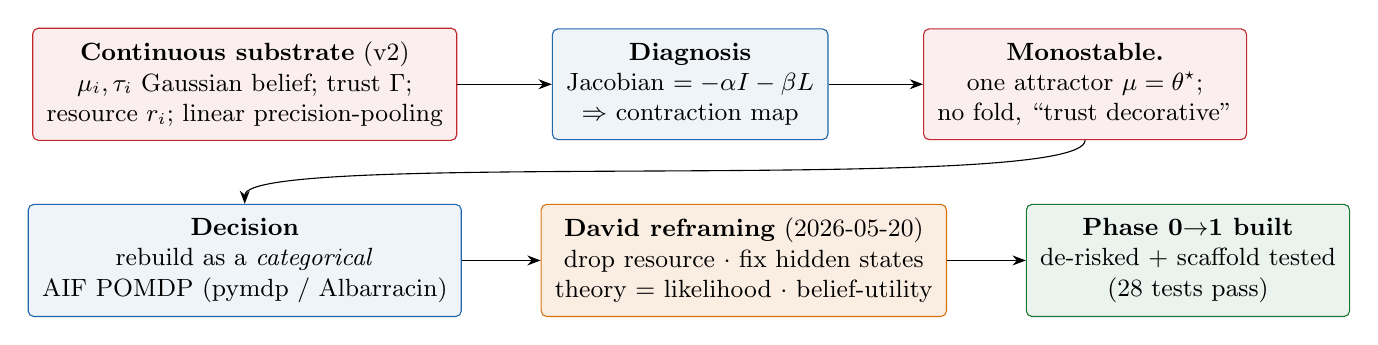
\begin{tikzpicture}[node distance=5.5mm]
\node[badbox] (old) {\textbf{Continuous substrate} (v2)\\
  $\mu_i,\tau_i$ Gaussian belief; trust $\Gamma$;\\ resource $r_i$; linear precision-pooling};
\node[box, right=12mm of old] (diag) {\textbf{Diagnosis}\\
  Jacobian $=-\alpha I-\beta L$\\ $\Rightarrow$ contraction map};
\node[badbox, right=12mm of diag] (mono) {\textbf{Monostable.}\\
  one attractor $\mu=\theta^\star$;\\ no fold, ``trust decorative''};
\draw[->] (old) -- (diag);
\draw[->] (diag) -- (mono);

\node[box, below=8mm of old] (dec) {\textbf{Decision}\\
  rebuild as a \emph{categorical}\\ AIF POMDP (pymdp / Albarracin)};
\node[fieldbox, right=10mm of dec] (david) {\textbf{David reframing} (2026-05-20)\\
  drop resource $\cdot$ fix hidden states\\
  theory $=$ likelihood $\cdot$ belief-utility};
\node[goodbox, right=10mm of david] (now) {\textbf{Phase 0$\to$1 built}\\
  de-risked $+$ scaffold tested\\ (28 tests pass)};
\draw[->] (mono.south) .. controls +(0,-0.7) and +(0,0.7) .. (dec.north);
\draw[->] (dec) -- (david);
\draw[->] (david) -- (now);
\end{tikzpicture}
\end{center}

\noindent The honest justification for going categorical is \emph{not} that it
was forced (the monostability proof is for the linearised reduction, and the
literature lists six bistability mechanisms). It is \textbf{strategic}:
literature alignment with Albarracin's ``Epistemic Communities'', and the POMDP
exposes the order parameters David asked for natively ($q(\theta)$, expected
free energy, $q(\pi)$).

% =====================================================================
\section*{2.\quad Old model vs.\ new model (what each object became)}
% =====================================================================
\begin{center}
\renewcommand{\arraystretch}{1.25}
\begin{tabular}{@{}p{4.3cm} p{5.0cm} p{5.0cm}@{}}
\toprule
 & \textbf{Old (continuous v2)} & \textbf{New (categorical POMDP)} \\
\midrule
belief over theory & Gaussian $\mu_i,\tau_i$ over $\theta\in\mathbb{R}$
   & categorical $q_i(\theta)$, $\theta\in\{A,B\}$ \\
how data is read & one shared regression likelihood
   & per-paradigm likelihood $A_\theta(o\mid s,a)$ \emph{(theory-ladenness)} \\
truth & moving target $\theta^\star(t)$
   & \textbf{fixed} state of nature; $B=$ identity \\
actions & choose experiment $x$ (info-gain)
   & choose experiment $a$ \emph{(measurement, not control)} \\
social coupling & linear precision-pool (DeGroot)
   & softmax-precision channel \emph{(folds, NB15)} \\
``mind-change'' / motivation & $\lambda\!\cdot\!U$ in the \emph{update} (blew up)
   & belief-utility $U(\theta)$ in the \emph{EFE/policy} \\
resource & $r_i$ flow + inflow (a state)
   & \textcolor{dropped}{\textbf{dropped}} (was a slaved readout) \\
\bottomrule
\end{tabular}
\end{center}

% =====================================================================
\section*{3.\quad The new generative model (one agent)}
% =====================================================================
\begin{center}
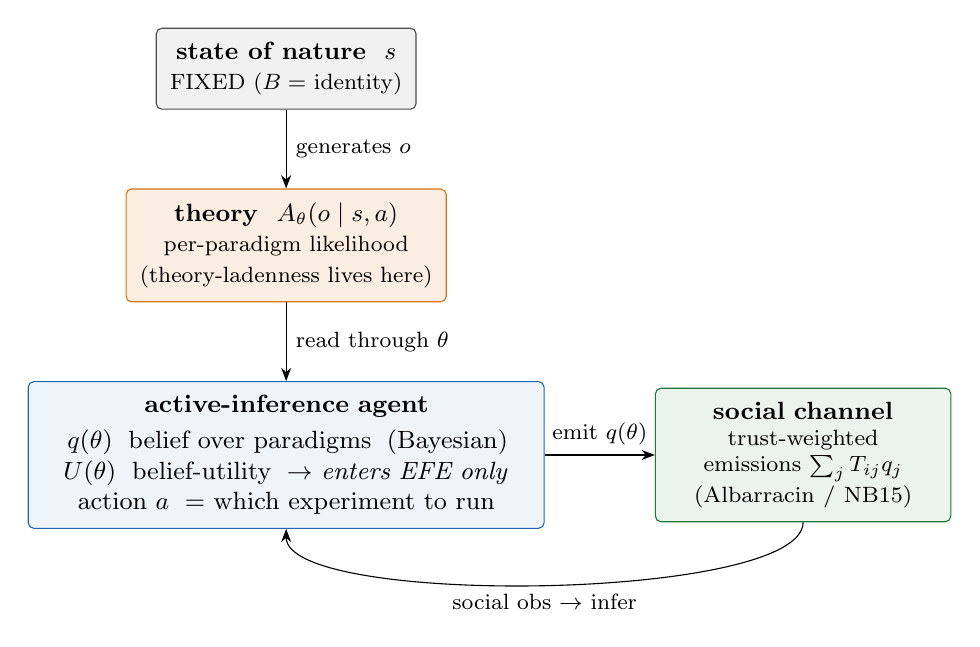
\begin{tikzpicture}[node distance=8mm]
\node[box, fill=neutralg!8, draw=neutralg] (s) {\textbf{state of nature } $s$\\
  \footnotesize FIXED ($B=$ identity)};
\node[fieldbox, below=10mm of s] (A) {\textbf{theory } $A_\theta(o\mid s,a)$\\
  \footnotesize per-paradigm likelihood\\ \footnotesize (theory-ladenness lives here)};
\node[box, below=10mm of A, text width=6.2cm] (agent)
  {\textbf{active-inference agent}\\[2pt]
   $q(\theta)$ \;belief over paradigms \;(Bayesian)\\
   $U(\theta)$ \;belief-utility \;$\to$ \emph{enters EFE only}\\
   action $a$ \;$=$ which experiment to run};
\node[goodbox, right=14mm of agent, text width=3.4cm] (soc)
  {\textbf{social channel}\\\footnotesize trust-weighted\\ \footnotesize emissions
   $\sum_j T_{ij}q_j$\\ \footnotesize (Albarracin / NB15)};

\draw[->] (s) -- node[right,font=\footnotesize]{generates $o$} (A);
\draw[->] (A) -- node[right,font=\footnotesize]{read through $\theta$} (agent);
\draw[->] (agent.east) -- node[above,font=\footnotesize]{emit $q(\theta)$} (soc.west);
\draw[->] (soc.south) .. controls +(0,-1.0) and +(0,-1.0) ..
   node[below,font=\footnotesize]{social obs $\to$ infer} (agent.south);
\end{tikzpicture}
\end{center}

\noindent\textbf{Two engines were meant to drive lock-in:} (i) \emph{motivated
sampling} --- $U(\theta)$ biases which experiments you run; (ii) \emph{social
reinforcement} --- the NB15 softmax-precision fold. Belief-utility heterogeneity
was meant to be the symmetry-breaking field turning polarization into
\emph{capture}. Section 5 is where that ran into a wall.

% =====================================================================
\section*{4.\quad What the four notebooks established}
% =====================================================================
\begin{center}
\begin{tikzpicture}[node distance=4mm and 9mm]
\node[badbox] (n14) {\textbf{NB14} Jacobian scan\\\footnotesize old substrate};
\node[goodbox, right=of n14] (n15) {\textbf{NB15} social fold\\\footnotesize go/no-go};
\node[goodbox, right=of n15] (n16) {\textbf{NB16} env-coupled fold\\\footnotesize the \emph{real} gate};
\node[box, right=of n16] (n17) {\textbf{NB17} scaffold\\\footnotesize Phase-1 smoke};

\node[below=2mm of n14, text width=3.3cm, font=\scriptsize, align=center]
  {$\rho\equiv0.9<1$ across the box; $\lambda U$ blows up. \textcolor{unstable}{Monostable confirmed.}};
\node[below=2mm of n15, text width=3.3cm, font=\scriptsize, align=center]
  {pitchfork at $K_c{=}2$. \textcolor{stable}{Categorical channel folds.} (env off)};
\node[below=2mm of n16, text width=3.5cm, font=\scriptsize, align=center]
  {fold survives \emph{iff} data underdetermined ($d$ small); belief-util tilts to capture. \textcolor{stable}{PASS w/ constraint.}};
\node[below=2mm of n17, text width=3.3cm, font=\scriptsize, align=center]
  {scaffold runs; regression holds; \textcolor{unstable}{martingale wall (\S5).}};
\draw[->] (n14)--(n15); \draw[->] (n15)--(n16); \draw[->] (n16)--(n17);
\end{tikzpicture}
\end{center}

% =====================================================================
\section*{5.\quad The Phase-1 finding: the martingale wall}
% =====================================================================
\begin{center}
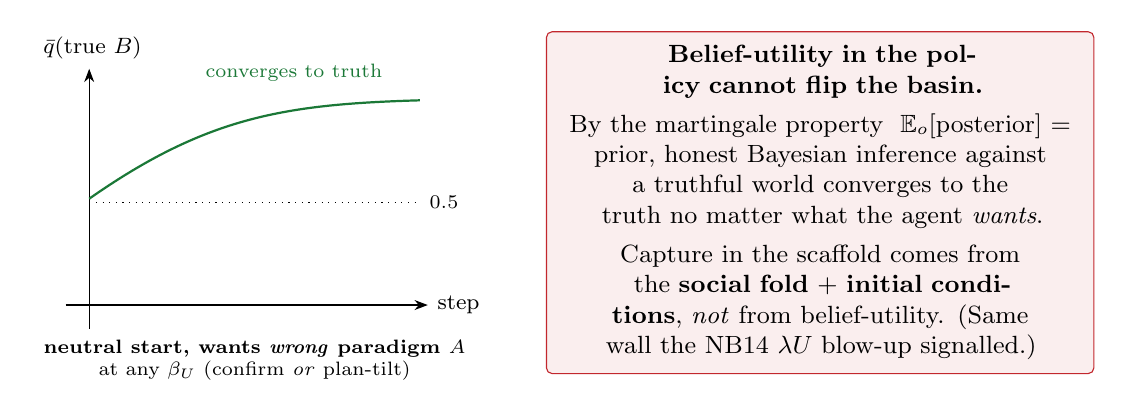
\begin{tikzpicture}
% left: the result
\begin{scope}
\draw[->] (-0.3,0) -- (4.3,0) node[right,font=\footnotesize]{step};
\draw[->] (0,-0.3) -- (0,3.0) node[above,font=\footnotesize]{$\;\bar q(\text{true }B)$};
\draw[dotted] (0,1.3) -- (4.2,1.3) node[right,font=\scriptsize]{$0.5$};
\draw[thick,stable] (0,1.35) .. controls (1.5,2.4) and (2.5,2.55) .. (4.2,2.6);
\node[stable,font=\scriptsize,align=center] at (2.6,2.95) {converges to truth};
\node[font=\scriptsize,align=center] at (2.1,-0.7)
  {\textbf{neutral start, wants \emph{wrong} paradigm $A$}\\ at any $\beta_U$ (confirm \emph{or} plan-tilt)};
\end{scope}
% right: the statement
\node[badbox, right=8mm of current bounding box.east, anchor=west,
      text width=6.6cm] at (5.0,1.3)
  {\textbf{Belief-utility in the policy cannot flip the basin.}\\[3pt]
   By the martingale property $\;\mathbb{E}_o[\text{posterior}]=\text{prior}$,
   honest Bayesian inference against a truthful world converges to the truth no
   matter what the agent \emph{wants}.\\[3pt]
   Capture in the scaffold comes from the \textbf{social fold $+$ initial
   conditions}, \emph{not} from belief-utility. (Same wall the NB14 $\lambda U$
   blow-up signalled.)};
\end{tikzpicture}
\end{center}

% =====================================================================
\section*{6.\quad The open decision (for you / David)}
% =====================================================================
\noindent Where should genuine \emph{capture-against-evidence} come from? The
scaffold supports all three with localised changes.
\begin{center}
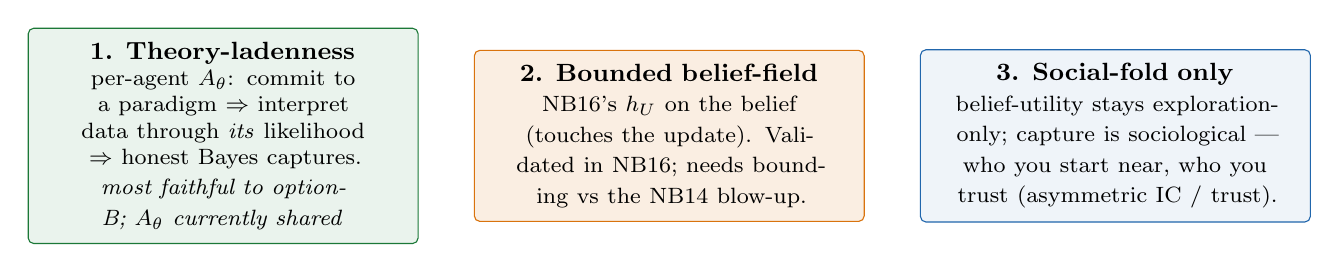
\begin{tikzpicture}[node distance=7mm]
\node[goodbox, text width=4.6cm] (o1)
  {\textbf{1. Theory-ladenness}\\\footnotesize per-agent $A_\theta$: commit to a
   paradigm $\Rightarrow$ interpret data through \emph{its} likelihood
   $\Rightarrow$ honest Bayes captures.\\ \footnotesize\emph{most faithful to
   option-B; $A_\theta$ currently shared}};
\node[fieldbox, right=of o1, text width=4.6cm] (o2)
  {\textbf{2. Bounded belief-field}\\\footnotesize NB16's $h_U$ on the belief
   (touches the update). Validated in NB16; needs bounding vs the NB14
   blow-up.};
\node[box, right=of o2, text width=4.6cm] (o3)
  {\textbf{3. Social-fold only}\\\footnotesize belief-utility stays
   exploration-only; capture is sociological --- who you start near, who you
   trust (asymmetric IC / trust).};
\end{tikzpicture}
\end{center}

\vspace{0.4em}
\noindent\textbf{Built this round (all in \texttt{src/pomdp/}, 28 tests pass):}
\texttt{gen\_model.py} (per-paradigm $A_\theta$, $B{=}$id, $C/D/U$),
\texttt{agent\_pop.py} (categorical AIF $+$ belief-utility EFE term, 3 modes),
\texttt{step.py} (emit$\to$route$\to$infer$\to$act),
\texttt{observables.py} (occupancy, EFE/$q(\pi)$, polarization, capture).
Notebooks \texttt{14--17}. Resource design archived in
\texttt{notes/archive/}. Full spec: \texttt{notes/pomdp\_generative\_model.md}.

\end{document}
